\chapter{CONCLUSIONS} 
\label{chapter:Conclusions}


% ----------------------- paths to graphics ------------------------


\ifpdf
    \graphicspath{{7_Conclusions/figures/PNG/}{7_Conclusions/figures/PDF/}{7_Conclusions/figures/}}
\else
    \graphicspath{{7_Conclusions/figures/EPS/}{7_Conclusions/figures/}}
\fi


% ----------------------- contents from here ------------------------
\section{Conclusions}
\noindent Now, we are capable of detecting the moving cars and capture the
over speeding cars to recognize the license plate of the car to send
it to the related authority. Another feature has been added to the
system, is to extract the Arabic numbers to send the license plate
contents to the related authority by sending an e-mail with an
attached text file which contains the Arabic numbers. This feature
will reduce the size of the attached file which will be sent to make
it easier and faster to be received by the related authority.

\section{ Future work:}
 \subsection{Professional cameras:}
\begin{enumerate}
	\item \textbf{Professional cameras for face detection:}\\
	Nowadays people are aware of the need of vehicle
	security due to the fact that they are various cases of car
	robbery. Therefore it is incumbent upon us to increase
	the level of securities. To make the system more secure,
	the system is recommended to integrate with face
	detection. This is means instead of identifying driver
	with their plate, it also important to identify by her or
	his face.\\
     We can do this by using a professional camera that
	contain a face detect applications, nowadays there are
	growing number of digital cameras now include a Face
	Recognition mode. The camera detects faces in a scene
	and then automatically focuses (AF) and optimizes
	exposure (AE).
	\item \textbf{- Professional camera to upgrade the image quality:}
	We want to use more professional cameras to improve
	the image quality to be easier to recognize the plate
	numbers.
	\begin{figure}[h]
		\centering
		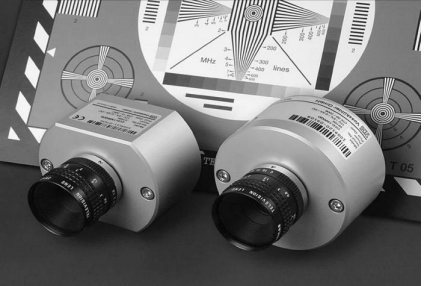
\includegraphics[width=0.45\textwidth]{figure2.png}
		\caption*{Color-ccd-digital camera	}
	\end{figure}
	\item \textbf{- Hard and waterproof cameras:}\\
	We can use hard cameras to avoid damages because
	they are located in the streets so they can be damaged
	by any one, but if we use hard material or it can be put
	in hard box it will be safer to avoid damage. Also, we
	want to use waterproof cameras because it is located in
	the open air, so maybe it will be rained.
	\item \textbf{Location of the camera:}\\
	The camera to vehicle distance around 40 feet. This
	system is able to detect license plate area for all the
	vehicles. We want to put the camera in the middle of
	the road to be able to detect any vehicles.
\end{enumerate}

\subsection{ Identification of segmented character:}
Save the segmented characters and numbers in one text file which
may be by comparing the segmented image with an already saved
one or compare it to a matrix of images in order to be ready for
database.
\begin{enumerate}
	\item \textbf{-Recognition System of Arabic Characters}\\
	At this stage, a recognition system of Arabic characters
	is presented, using a structural method based on the
	extraction of primitives (holes, concavities, characters
	form, existence of points, position of point, and number
	of connected components). This stage is performed in
	two steps;
	Characters classification and identification.\\
	\uline{\textbf{a$)$ Characters classification:}}\\
	The character classification takes as criteria the
	concavities in different directions, and the holes, which
	represent the main characteristics (morphological ones).
	The choice of these characteristics enables the system
	to work with multi-sized characters without having to
	perform an eventual normalization.
\end{enumerate}
\noindent The inner details of characters such as the presence of holes and
concavities are obtained to produce some unique features for some
Arabic characters. The holes feature is used to identify some
characters or resolve any ambiguity in the recognition phase. The
presence or absence of the hole, concavities direction, and dots are
powerful features for enhancing the implemented Arabic
recognition system. 

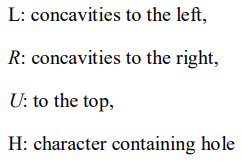
\includegraphics{ff.png}\\
We can compute each character's class using this formula:
\begin{equation*}
	class=2^0H+2^1U+2^2R+2^3L
\end{equation*}

\begin{figure}[h]
	\centering
    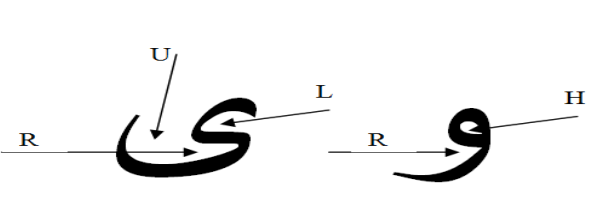
\includegraphics[width=0.5\textwidth]{aa.png}
\end{figure}

We must study the intensity of top and down parts, if the character
has the intensity of top part is smaller or greater than the intensity
of the down part. 
\begin{figure}[h]
	\centering
	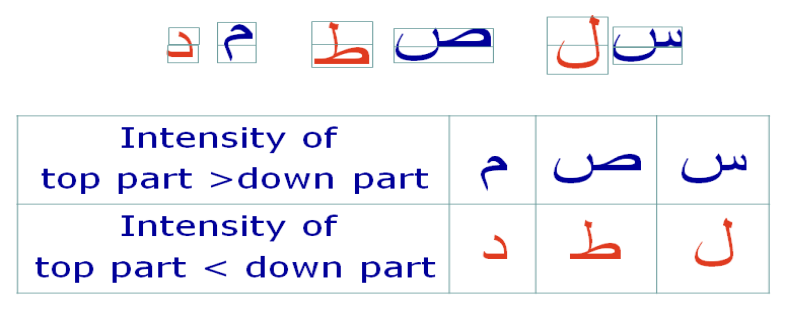
\includegraphics[width=0.6\textwidth]{bb.png}
\end{figure}
\\
\uline{\textbf{b$)$Characters identification:}}\\
-Egyptian new license plates use only 17 characters
from 28.
\begin{figure}[h]
	\centering
	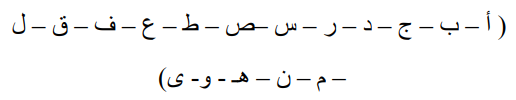
\includegraphics[width=0.5\textwidth]{ee.png}
	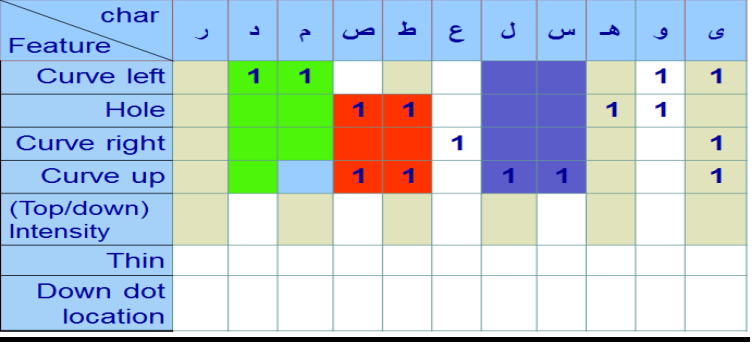
\includegraphics[width=0.7\textwidth]{cc.png}
	\caption*{After that we can identify any Arabic plate character.}
\end{figure}
\subsection{Creating a database of the system:}
We use to create a data base for all the cars plate numbers and their
owner identity .We use SQL to create a database for the car plate
number and the name of the owner and his penalty.
\begin{figure}[!h]
	\centering
	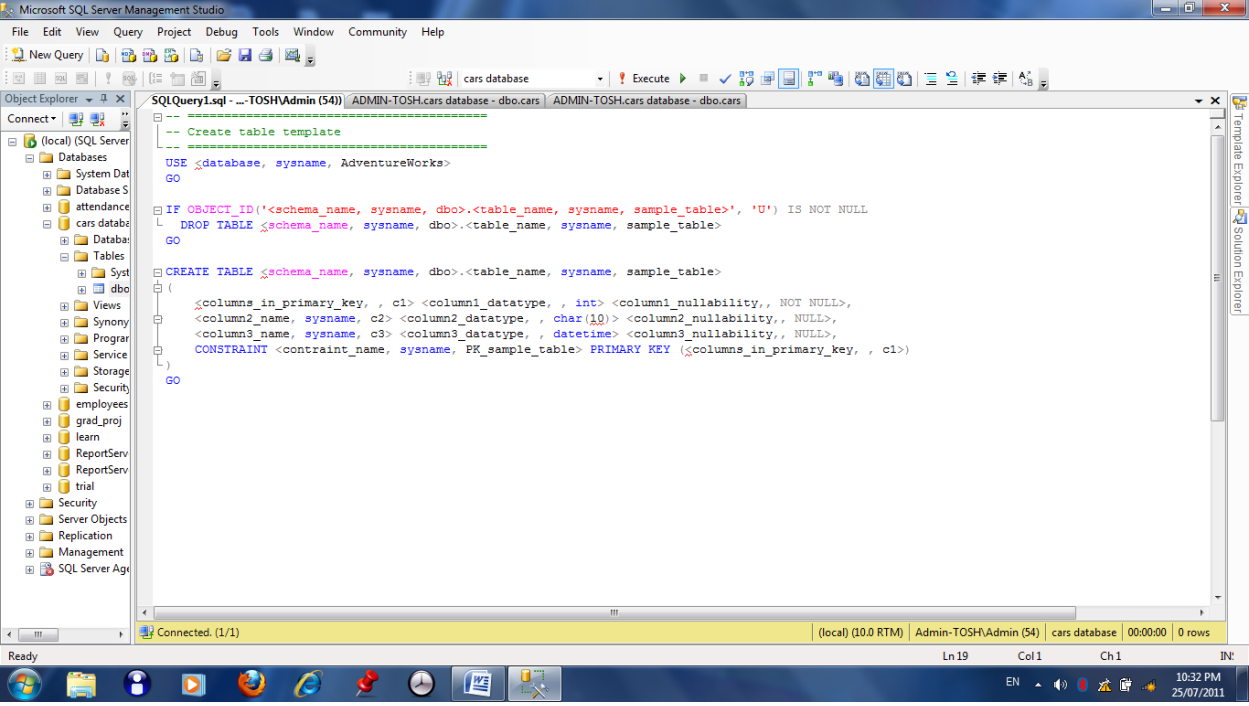
\includegraphics[width=0.64\textwidth]{dd.png}
\end{figure}
\subsection{Sending SMS}
\noindent After building the database system and detecting the license plate
numbers, we will use these numbers to compare it with the data
base elements to extract the car owner's telephone number. After
that we will use a software program to send an automatic SMS to
the car owner to inform him that he has been crossed the limit
speed. This program will be designed by C\# and the main function
of the operation will be:\\
\textcolor{red}{sms = "You've received a speeding ticket!$\backslash$nSpeed: " + 150 +
	"$\backslash$nPlace: Alexandrai ST @ 100 KM$\backslash$nTime: " + DateTime.Now + "$\backslash$nBill: "
	+ 500 + " LE";\\
	sendSMS("COM19", "0105471662", sms);} \\
We have first to attach the mobile phone to the COM port, and
defining it by task manager. Then the SMS will be sent to the
required number via the attached mobile phone.
\subsection{Moving and non moving cars}
\noindent Use the LPR (license Plate Recognition) in monitoring roads and
detect moving parts by using video segmentation this system is
used in south Africa where we can catch stolen cars by
automatically recognize the car plate and search it in a database, if
the passing car is identical with one of those in the black list it
sends the location to the authorized persons. Detection of moving
vehicles simplifies the processing on subsequent analysis steps.
Due to dynamic changes in natural scenes such as sudden
illumination and weather changes, repetitive motions that cause
clutter (tree leaves moving in blowing wind), motion detection is a
difficult problem to process reliably. Frequently used techniques
for moving vehicle detection are background subtraction, statistical
methods, temporal differencing and optical flow. In case we used
the Background subtraction which is particularly a commonly used
technique for motion segmentation in static scenes, it attempts to
detect moving regions by subtracting the current image pixel-bypixel from a reference background image that is created by
averaging images over time in an initialization period, The pixels
where the difference is above a threshold are classified as
foreground. After creating a foreground pixel map, some
morphological post processing operations such as erosion, dilation
and closing are performed to reduce the effects of noise and
enhance the detected regions. The reference background is updated
with new images over time to adapt to dynamic scene changes.
While in case we used Statistical Methods which is more advanced
methods that make use of the statistical characteristics of
individual pixels have been developed to overcome the
shortcomings of basic background subtraction methods. These
statistical methods are mainly inspired by the background
subtraction methods in terms of keeping and dynamically updating
statistics of the pixels that belong to the background image
process. Foreground pixels are identified by comparing each
pixel's statistics with that of the background model. This approach
is becoming more popular due to its reliability in scenes that
contain noise, illumination changes and shadow Finally both
methods can detect the moving vehicle we can use one of them to
reach our target and distinguish between the moving cars and the
non-moving ones for any following purposes.


% ---------------------------------------------------------------------------
% ----------------------- end of thesis sub-document ------------------------
% --------------------------------------------------------------------------- 